\documentclass[compress]{beamer}
\usepackage{ifthen,verbatim}

\title{Track-based alignment \\ of the CMS muon detector}
\author{Jim Pivarski, Alexei Safonov}
\institute{Texas A\&M University}
\date{12 April, 2008}

\newcommand{\isnote}{}
\xdefinecolor{lightyellow}{rgb}{1.,1.,0.25}
\xdefinecolor{darkblue}{rgb}{0.1,0.1,0.7}

%% Uncomment this to get annotations
%% \def\notes{\addtocounter{page}{-1}
%%            \renewcommand{\isnote}{*}
%% 	   \beamertemplateshadingbackground{lightyellow}{white}
%%            \begin{frame}
%%            \frametitle{Notes for the previous page (page \insertpagenumber)}
%%            \itemize}
%% \def\endnotes{\enditemize
%% 	      \end{frame}
%%               \beamertemplateshadingbackground{white}{white}
%%               \renewcommand{\isnote}{}}

%% Uncomment this to not get annotations
\def\notes{\comment}
\def\endnotes{\endcomment}

\setbeamertemplate{navigation symbols}{}
\setbeamertemplate{headline}{\mbox{ } \hfill
\begin{minipage}{5.5 cm}
\vspace{-0.75 cm} \small
\end{minipage} \hfill
\begin{minipage}{4.5 cm}
\vspace{-0.75 cm} \small
\begin{flushright}
\ifthenelse{\equal{\insertpagenumber}{1}}{}{Jim Pivarski \hspace{0.2 cm} \insertpagenumber\isnote/\pageref{numpages}}
\end{flushright}
\end{minipage}\mbox{\hspace{0.2 cm}}\includegraphics[height=1 cm]{../cmslogo} \hspace{0.1 cm} \includegraphics[height=1 cm]{../tamulogo} \hspace{0.01 cm} \vspace{-1.05 cm}}

\begin{document}
\begin{frame}
\begin{center}
\textcolor{darkblue}{\LARGE Track-based alignment \\ of the CMS muon detector}

\vfill \vfill \includegraphics[width=0.6\linewidth]{sun_shines_in_the_muon_barrel.jpg}

\end{center}
\begin{columns}
\column{0.5\linewidth}
\begin{center}
\textcolor{darkblue}{Jim Pivarski,} Alexei Safonov

\small Texas A\&M University
\end{center}

\column{0.5\linewidth}
\begin{center}
\scriptsize American Physical Society April Meeting

April 12, 2008 (B12.00006)
\end{center}
\end{columns}
\end{frame}

% 1. cms detector, highlighting muon system: muon sees 24 (high eta) - 44 (barrel) layers (a complete tracking system in itself!)
% 1.5 muon barrel consists of 250 drift tube chambers, endcap 540 cathode strip chambers (diagram)
% 2. relative precision of tracker (10-50 microns: PTDR sec6.6) and muon systems (200 microns fig3.27): muon system matters for track resolution at TeV energies
% 3. modular detector (lowering disk), iron bends in magnetic field: chambers mounted on joints to avoid twisting chambers (chambers are rigid bodies, but orientation is unknown)
% 4. system of lasers and calipers mounted on chambers to monitor positions: observed expected deflections due to magnet in assembly hall on surface in 2006, everything taken apart and lowered into cavern, will be measured again later this month

\begin{frame}
\frametitle{CMS muon tracking system}

\vfill \vfill Outermost part of the Compact {\it Muon} Solenoid (CMS)

\includegraphics[width=\linewidth]{cms_slice.png}

\vfill\vfill\begin{itemize}
\item Typical muon leaves a trail of 24--44 hits in muon system
\item A complete tracking system in itself!
\item Measure muon momentum by curvature of its 7-meter \mbox{long track\hspace{-1 cm}}
\end{itemize}
\end{frame}

\begin{frame}
\frametitle{Independent components}
\begin{columns}
\column{0.4\linewidth}
\includegraphics[width=\linewidth]{lowering2.jpg}
\column{0.7\linewidth}

\begin{center}
\includegraphics[width=0.8\linewidth]{modularity.png}
\end{center}

\vspace{-0.5 cm}
\begin{itemize}
\item Built in an assembly hall and lowered, piece by piece, to the interaction point
\item Iron disks shift and bend centimeters in CMS's 4-Tesla magnetic field
\item 790 chambers mounted on ball-joints to remain internally rigid
\end{itemize}

\vspace{0.25 cm}
\hfill \begin{minipage}{0.95\linewidth}
Hit resolution depends on precise knowledge of chambers' position and orientation in space
\end{minipage} \hfill \mbox{ }

\end{columns}
\end{frame}

\begin{frame}
\frametitle{Does muon alignment matter?}

\begin{itemize}\setlength{\itemsep}{0.25 cm}
\item Triggering and muon-id are insensitive to misalignment, \mbox{by design\hspace{-1 cm}}

\item Inner tracker dominates in $p_T$ resolution because hits are $\sim$10~times more precise
\begin{itemize}
\item Inner tracker: 10--50~$\mu$m silicon strip measurements
\item Muon chamber: 200~$\mu$m drift tubes and cathode strips
\end{itemize}

\uncover<2>{\hspace{-0.75 cm} \ldots but only below 1~TeV
\begin{center}
\begin{minipage}{0.7\linewidth}
\begin{columns}
\column{0.5\linewidth}
\includegraphics[width=\linewidth]{Figure_001-005-a.pdf}
\column{0.5\linewidth}
\includegraphics[width=\linewidth]{Figure_001-005-b.pdf}
\end{columns}
\end{minipage}
\end{center}}

\item<2> TeV tracks are so straight that muon system's lever arm
contributes significantly to momentum resolution: it matters!
\end{itemize}
\end{frame}

\begin{notes}
\item This page will not be in the final talk
\item tracker's 10-50 microns comes from PTDR section 6.6 (but
majority of hits are in the 15-30 range, that's why I say 10 times the
precision)
\item muon systems's 200 microns comes from PTDR Figure 3.27 (doesn't
include CSC wire measurement which has centimeter uncertainties in
spatial resolution (but good timing))
\item these two plots are figures 001-005-a and b
\end{notes}

\begin{frame}
\frametitle{Hardware alignment system}

System of lasers and calipers mounted on chambers

\vfill Measure positions and monitor changes

\vfill \includegraphics[width=\linewidth]{hardware_alignment.png}
\end{frame}

% 5. track-based alignment: correct assumed chamber positions by minimizing track - hit residuals
%     aligns active elements directly, rather than the boxes they live in
%     chamber parameter resolution is proportional to how sensitive track-fitting is to those parameters, i.e. how much it matters
%     usually this is a chicken-and-egg problem: tracks are fit by minimizing residuals w.r.t. the hits!
%         problem solved by global fit (Blobel's MillePede, Kalman-based) or iteration
%     different problem in muon system: track measured precisely by inner tracking system, but scatters in material
%         solved by identifying highly-scattering tracks using muon system redundancy (implicit: that's something ATLAS can't do)
%         and local track-fitting

\begin{frame}
\frametitle{Track-based alignment}

\begin{columns}
\column{0.3\linewidth}
\only<1>{\includegraphics[width=\linewidth]{track_based_alignment2.png}}\only<2->{\includegraphics[width=\linewidth]{track_based_alignment.png}}
\column{0.7\linewidth}
Find corrections to assumed chamber positions by minimizing track-minus-hit residuals
\end{columns}

\vfill
\begin{itemize}
\item Independent alternative to Muon Hardware Alignment System
\item Aligns active sensors directly, rather than the boxes they live in
\item Parameter resolution is proportional to \mbox{sensitivity of track-fitting:\hspace{-1 cm}}

best resolution on the parameters \mbox{that matter most\hspace{-1 cm}}
\end{itemize}

\vfill \hspace{-0.83 cm} \uncover<3-4>{\textcolor{darkblue}{\Large Challenges and solutions}}

\begin{itemize}
\item<3-4> Ordinarily, a chicken-and-egg problem: tracks are fit by minimizing residuals, too!
\begin{itemize}
\item We can use the inner silicon tracker as a reference
\end{itemize}
\item<4> Muon system has a lot of iron: multiple-scattering \mbox{distorts track\hspace{-1 cm}}
\begin{enumerate}
\item Remove highly scattering tracks from sample
\item Re-fit tracks using local information
\end{enumerate}
\end{itemize}
\end{frame}

% 6. track scattering schematic and local fitting
%     scattering effects are antisymmetric w.r.t. charge, depend on momentum
%     local fit inner chambers, work outward
%     some chambers overlap slightly with no iron in between: local-fit tracks in these regions for relative alignments

\begin{frame}
\frametitle{Muon Alignment Techniques}

\begin{columns}
\column{0.35\linewidth}
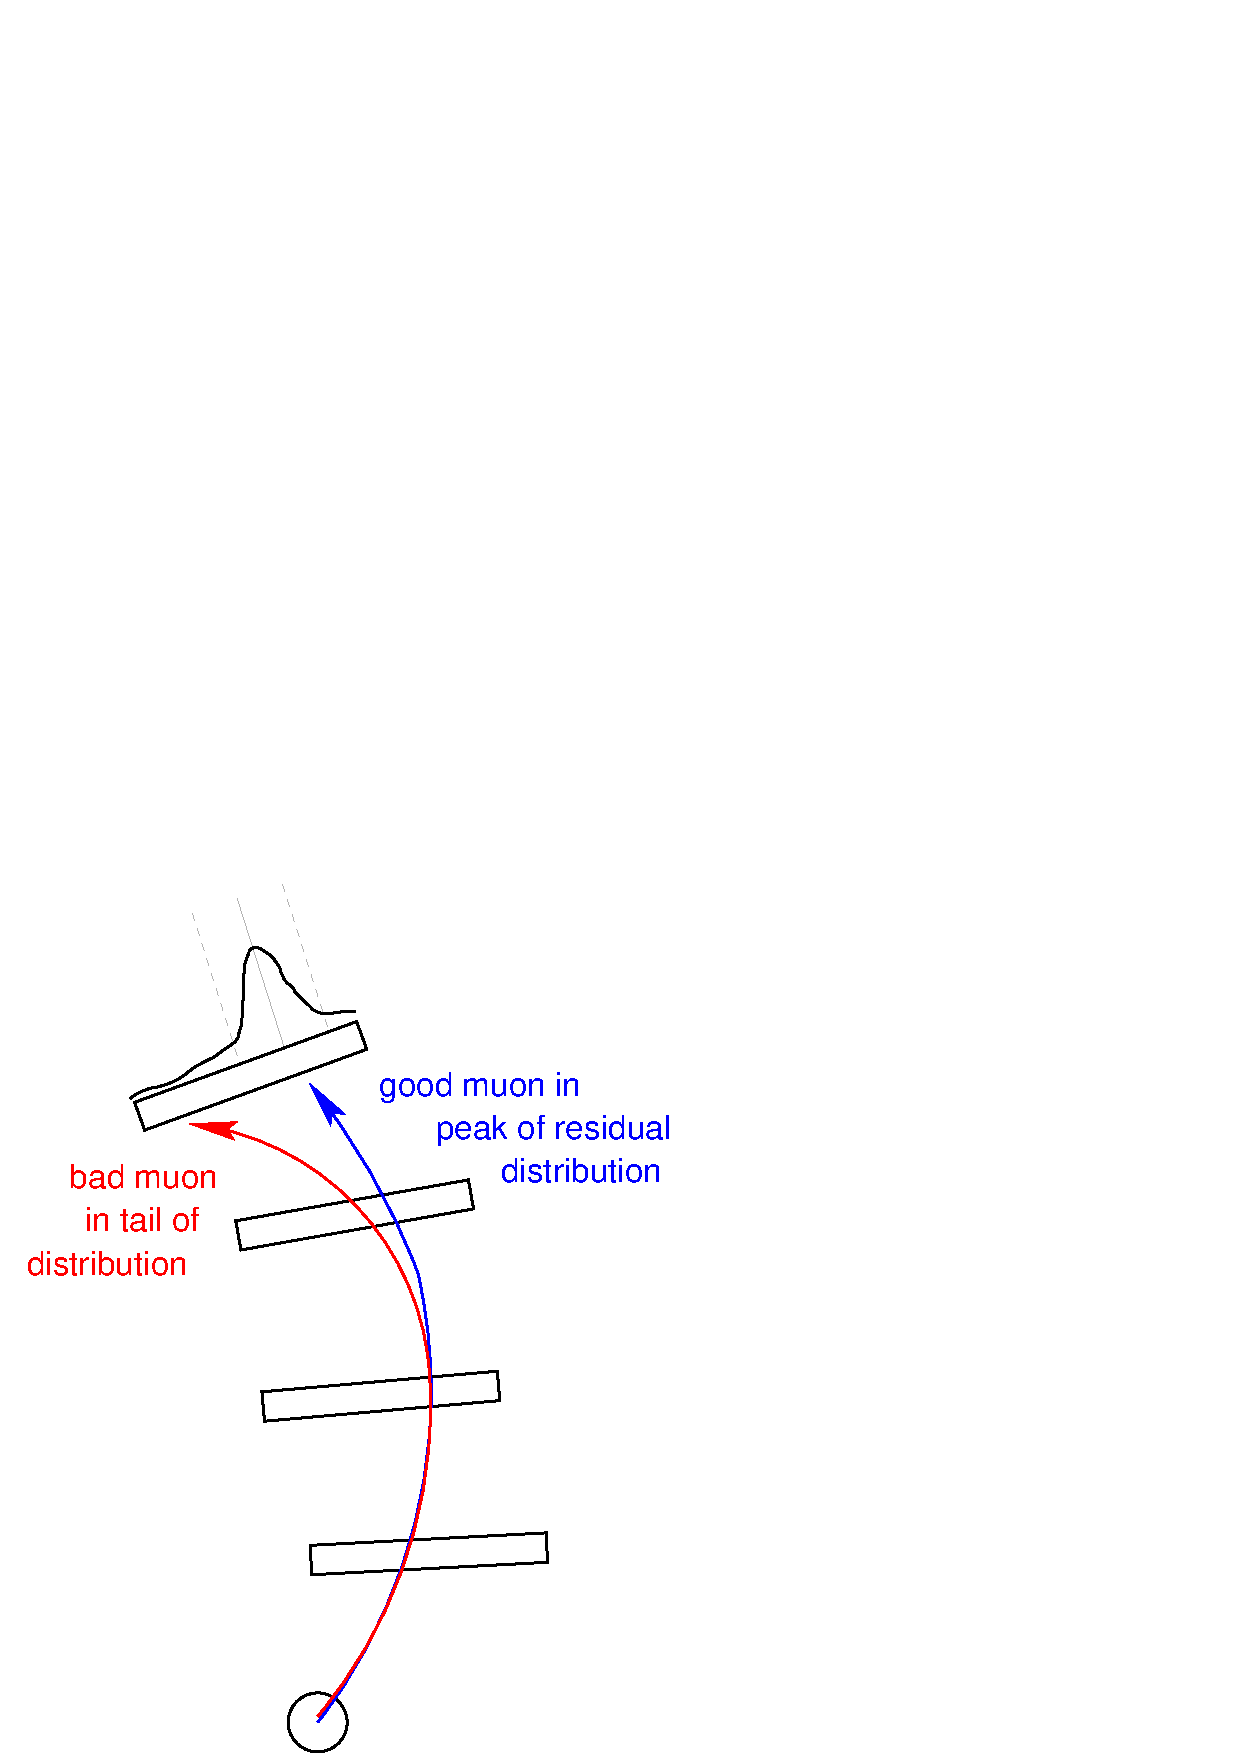
\includegraphics[width=1.285\linewidth]{trackcut.pdf}

\column{0.65\linewidth}
\begin{itemize}
\item Use redundancy of muon system to identify multiply-scattering
tracks
\begin{itemize}
\item Scattered tracks are in tails of the residual distributions
\item Dozens of residual distributions per track: one for each layer hit
\end{itemize}

\item Scattering bias is antisymmetric with charge, only affects low momentum

\item<2-3> Local track-fitting:
\begin{itemize}
\item Re-fit tracks with all but a few hits deweighted (inflated uncertainty)

\end{itemize}

\end{itemize}
\end{columns}

\vspace{-0.3 cm}
\begin{columns}
\column{0.15\linewidth}
\uncover<3>{\includegraphics[width=1.1\linewidth]{overlap.png}}
\column{0.6\linewidth}
\begin{itemize}
\item<3> Some chambers overlap without intervening iron layer
\begin{itemize}
\item local-fit shared track segment
\item align chambers relative to one another
\end{itemize}
\end{itemize}
\column{0.3\linewidth}

\vspace{-1 cm}
\uncover<2-3>{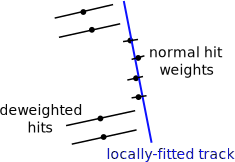
\includegraphics[width=\linewidth]{loose_hits.png}}

\vspace{-1 cm}
\mbox{ }
\end{columns}
\end{frame}

% 7. start-up alignment methods: cosmic rays for barrel, beam-halo for endcap (this spring: before colliding beams!)
%     strategy: (1) do relative chamber alignments within modular structures using cosmics, beam-halo
%               (2) align large modular structures to inner tracking system with the first few weeks of collisions
% 8. simulated effects of misalignment on physics: 1-2 TeV Z' (PAS of analysis note)
% 9. conclusions

\begin{frame}
\frametitle{Start-up alignment methods}

\begin{tabular}{c c}
\includegraphics[height=3.5 cm]{cosmics.pdf} & \includegraphics[height=3.5 cm]{beamhalo.pdf} \\
Cosmic rays for barrel & Beam-halo for endcaps
\end{tabular}

\vfill \vfill \textcolor{darkblue}{Strategy:}
\begin{enumerate}
\item Find relative chamber alignments within modular structures (barrel wheels and endcap disks) using cosmics, beam-halo
\item Align modular structures to inner tracker with first collisions
\begin{itemize}
\item These structures cover large solid angles
\item Not many tracks are needed for a precise alignment
\end{itemize}
\end{enumerate}
\end{frame}

\begin{frame}
\frametitle{TeV dimuons with misalignment}

Simulated $Z'$ peak shape with residual misalignment

\vfill \includegraphics[width=\linewidth]{misaligned_spectra.png}

\textcolor{blue}{Misaligned muon system} matters a lot more at 2~TeV, as expected
\end{frame}

\begin{notes}
\item This page will not be in the final talk
\item The plot on the previous page is in the PAS of analysis note 2007/038 (figure 3 of PAS version 3), so it's public
\item {\tt \small http://cms.cern.ch/iCMS/analysisadmin/viewanalysis?

id=29\&field=id\&value=29\&name=TeVMu\%202007

\%20Analysis\%20effort}
\end{notes}

\begin{frame}
\frametitle{Conclusions}
\large
\begin{itemize}\setlength{\itemsep}{0.7 cm}
\item CMS muon detector is a many-layered tracking system
\item Modular structure requires alignment
\item Track-based alignment poses a unique set of challenges in this environment
\item Significant impact on early physics: width of $Z'$ resonance
\end{itemize}
\label{numpages}
\end{frame}

%% \begin{notes}
%% \item This is the annotated version of my talk.
%% \item If you want the version that I am presenting, download the one
%% labeled ``slides'' on Indico (or just ignore these yellow pages).
%% \item The annotated version is provided for extra detail and a written
%% record of comments that I intend to make orally.
%% \item Yellow notes refer to the content on the {\it previous} page.
%% \item All other slides are identical for the two versions.
%% \end{notes}

%% \begin{frame}
%% \frametitle{Outline}
%% \begin{itemize}\setlength{\itemsep}{0.75 cm}
%% \item 
%% \end{itemize}
%% %% \hspace{-0.83 cm} \textcolor{darkblue}{\Large Outline2}
%% \end{frame}

%% \section*{First section}
%% \begin{frame}
%% \begin{center}
%% \Huge \textcolor{blue}{First section}
%% \end{center}
%% \end{frame}

\end{document}
